

\author[Jannis Klingler]{Nix}


\beamertemplatenavigationsymbolsempty{}

\logo{
\includegraphics[height=1cm]{Bilder/logo}}



\section{Variational Autoencoder}

\begin{frame}
	\frametitle{Beispiel \emph{time series}}
	\begin{figure}[!htbp]
		
\includegraphics[scale=0.25]{Bilder/rotatingMNIST}
		\caption{Beispiel einer \emph{time series} bestehend aus \\10 Bildern des Datensatzes rotatingMNIST}
	\end{figure}
\end{frame}

\begin{frame}
	\frametitle{Modellannahmen}
	Datensatz $\textbf{X} = \lbrace\x \rbrace_{i=1}^{N} \subset \R^{D\times N}$\\
	Datenpunkte $\x\sim p(\x)$ (u.i.v. Realisierungen einer hochdimensionalen ZV)
\end{frame}

\begin{frame}
	\frametitle{Schematische Darstellung der VAE-Architektur}
	\begin{figure}[htbp!]
		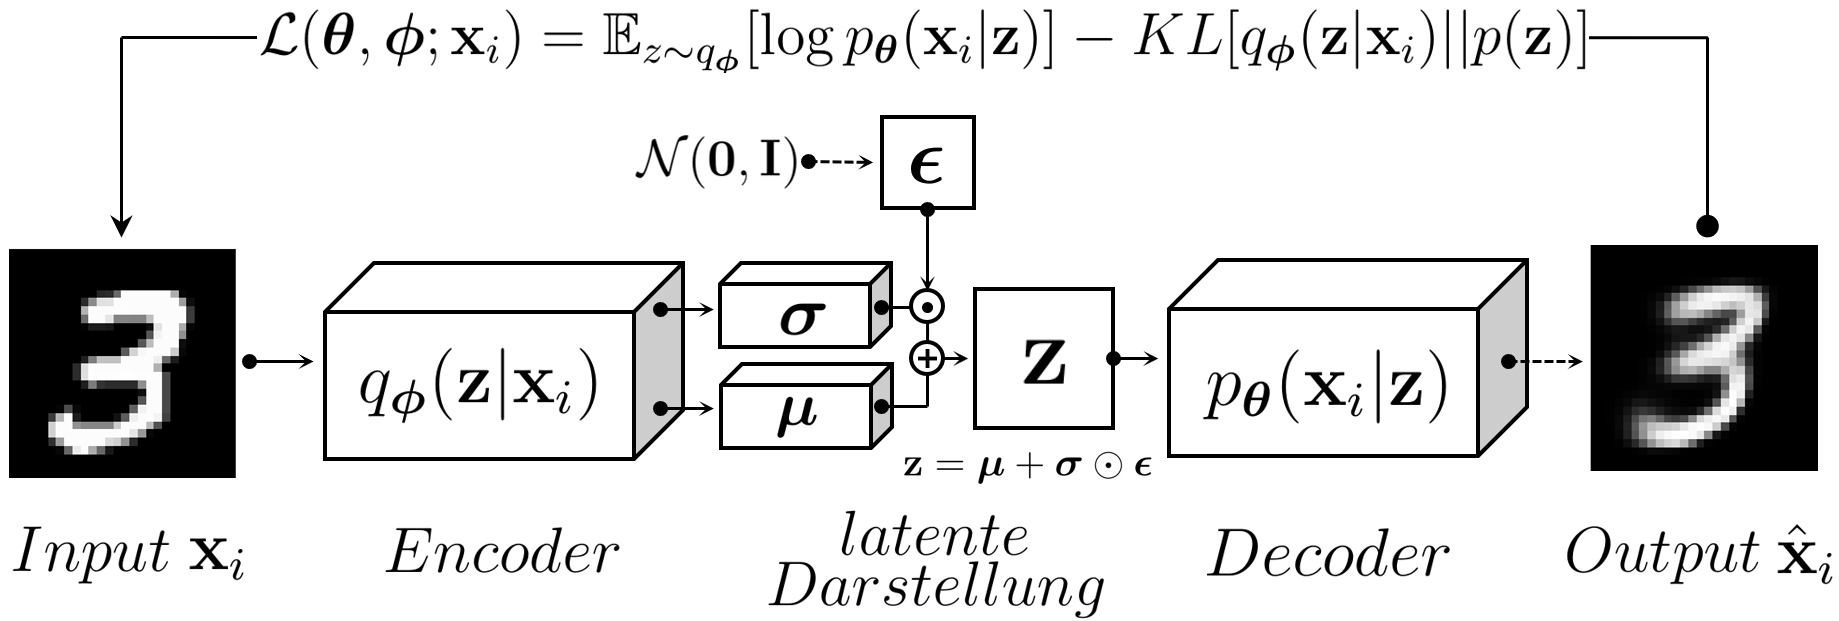
\includegraphics[scale=0.27]{Bilder/VAE-Modell.PNG}
	\end{figure}
\end{frame}